\documentclass[10pt,twocolumn,letterpaper]{article}

\usepackage{cvpr}
\usepackage{times}
\usepackage{epsfig}
\usepackage{graphicx}
\usepackage{amsmath}
\usepackage{amssymb}
\usepackage{listings}
\usepackage{xcolor}
\usepackage[table,xcdraw]{xcolor}
\usepackage{caption}
\usepackage{makecell}
\usepackage[T1]{fontenc}
\usepackage{placeins}
\usepackage{booktabs}

\definecolor{lightergray}{rgb}{0.9,0.9,0.9}
\renewcommand{\arraystretch}{1.15}
\captionsetup[table]{skip=5pt}

\lstset{
    language=Python,
    basicstyle=\ttfamily\small,
    keywordstyle=\color{blue},
    stringstyle=\color{red},
    commentstyle=\color{green},
    showstringspaces=false,
    frame=single,
    breaklines=true
}
% Include other packages here, before hyperref.

% If you comment hyperref and then uncomment it, you should delete
% egpaper.aux before re-running latex.  (Or just hit 'q' on the first latex
% run, let it finish, and you should be clear).
\usepackage[breaklinks=true,bookmarks=false]{hyperref}

\cvprfinalcopy % *** Uncomment this line for the final submission

\def\cvprPaperID{****} % *** Enter the CVPR Paper ID here
\def\httilde{\mbox{\tt\raisebox{-.5ex}{\symbol{126}}}}

% Pages are numbered in submission mode, and unnumbered in camera-ready
%\ifcvprfinal\pagestyle{empty}\fi
\setcounter{page}{1}
\begin{document}

%%%%%%%%% TITLE
\title{A Neural Network Approach to Classification of Protein Residue Interactions}

\author{Andrea Auletta\\
{\tt\small andrea.auletta@studenti.unipd.it}
% For a paper whose authors are all at the same institution,
% omit the following lines up until the closing ``}''.
% Additional authors and addresses can be added with ``\and'',
% just like the second author.
% To save space, use either the email address or home page, not both
\and
Marco Bernardi\\
{\tt\small marco.bernardi.11@studenti.unipd.it}
\and
Niccolò Zenaro\\
{\tt\small niccolo.zenaro@studenti.unipd.it}
}

\maketitle
%\thispagestyle{empty}

\begin{abstract}
    This paper presents a machine learning approach to classify protein residue interactions within the framework of Residue Interaction Networks (RINs). 
    Utilizing the RING tool, we obtained a dataset containing over 2.4 million residue-residue contacts, categorized into several interaction types. Given the inherent class imbalance in the dataset, with a significant overrepresentation of certain interaction types such as hydrogen bonds and van der Waals interactions, multiple techniques were explored to address this imbalance. 
    These included undersampling, oversampling using the Synthetic Minority Over-sampling Technique (SMOTE), and class merging strategies. We implemented and compared several models, including XGBoost and neural networks, focusing on their ability to accurately predict the interaction type. 
    The challenges posed by the overlap of classes in the feature space are discussed, alongside the preprocessing steps taken to enhance model performance. 
    The results of our analysis highlight the effectiveness of the proposed methods and provide insights into the complexities of classifying protein residue interactions.
\end{abstract}
    

%%%%%%%%% BODY TEXT
\section{Introduction}

Residue Interaction Networks (RINs) are a representation of the non-covalent interactions between amino acid residues within a protein structure, derived based on their geometrical and physico-chemical properties. These networks provide a detailed mapping of intra-protein contacts, which are crucial for understanding the structural and functional dynamics of proteins. 
RING (\url{https://ring.biocomputingup.it/}) is a computational tool that facilitates the analysis of these networks by processing Protein Data Bank (PDB) files (\url{https://www.rcsb.org/}) to identify and classify residue-residue interactions within a given protein structure. 
RING categorizes these interactions into distinct contact types, including Hydrogen Bonds (HBOND), Van der Waals interactions (VDW), Disulfide Bridges (SBOND), Salt Bridges (IONIC), $\pi$-$\pi$ Stacking (PIPISTACK), $\pi$-Cation Interactions (PICATION), Hydrogen-Halogen Interactions (HALOGEN), Metal Ion Coordination (METAL\_ION), $\pi$-Hydrogen Bonds (PIHBOND), and a category for Unclassified Contacts.

This project is centered around the development of a predictive model that can infer the RING classification of residue contacts using statistical or supervised learning approaches, as opposed to purely geometrical methods. The objective is to design a program that calculates the likelihood or propensity of a residue-residue interaction belonging to each contact type defined by RING, starting from the structural data of the protein.


\section{Data Source}
\label{sec:datasource}

The dataset utilized in this study comprises a collection of training examples derived from 3,299 Protein Data Bank (PDB) structures. Each PDB structure is represented by a separate file, which provides detailed information on the residue-residue contacts identified within the corresponding protein. The files are available for download and are organized such that each file contains a tab-separated table of interactions for a single PDB structure. 

Across all 3,299 PDB structures, the dataset contains a total of 2,476,056 residue-residue contacts, distributed among various interaction types as represented in the table below \ref{ref:DatasetDistribution}.

\begin{table}[h!]
    \centering
    \begin{tabular}{|l|r|}
    \hline
    \textbf{Contact Type} & \textbf{Count} \\
    \hline
    HBOND & 901.814 \\
    VDW & 640.469 \\
    PIPISTACK & 32.965 \\
    IONIC & 30.355 \\
    SSBOND & 1.792 \\
    PICATION & 7.623 \\
    PIHBOND & 1.836 \\
    Unclassified & 860202 \\
    \hline
    \end{tabular}
    \caption{Distribution of contact types across the dataset.}
    \label{ref:DatasetDistribution}
\end{table}

Each file is formatted as a tab-separated table, consisting of columns that provide essential details for each contact. The columns include residue identifiers, which follow the same naming conventions as those used in BioPython, along with several pre-calculated features. The final column in each table specifies the type of interaction, categorizing the contact according to the RING-defined classifications.

\subsection{Data Preprocessing}

The files containing the information for each PDB structure were merged into a single dataframe, creating the dataset for the model. This dataset underwent a preprocessing phase, which involved several crucial steps for data cleaning and preparation.

First, the null values present in the dataset were replaced with the mean of the corresponding column values. This operation ensured data continuity, minimizing the impact of missing values on the model's performance.

Furthermore, all rows lacking a classification, i.e., without a value in the "interaction" column, were reclassified under the "Unclassified" category. This update involved modifying the values in the "interaction" column, ensuring that every interaction in the dataset was consistently labeled according to the contact categories defined by RING.

%Qui bisogna dire anche le feature che abbiamo usato e come le abbiamo preprocessate. (secondary structure)

\section{Approaches}
\subsection{Balancing the Dataset}
As observed in Section \ref{sec:datasource}, the dataset exhibits a significant imbalance, with a disproportionately large number of HBOND, VDW, and Unclassified interactions compared to the other contact types. 
Various techniques have been employed to address this imbalance, and these methods are detailed in the subsequent sections.
\paragraph{Undersampling}
The dataset was balanced by reducing the number of samples in the classes with a higher frequency to match the size of the class with the fewest samples, or to a lower, predefined number. 
This reduction was performed randomly. However, this approach presents the drawback of discarding a substantial amount of data, which may result in the model's inability to fully learn the distinguishing features of the classes with a larger number of samples.

\paragraph{Oversampling - SMOTE}
The Synthetic Minority Over-sampling Technique (SMOTE)\cite{chawla2002smote} was applied to generate synthetic samples for the minority classes, thereby increasing their representation in the dataset. 
This method involves calculating the difference between a sample and its nearest neighbors, multiplying this difference by a random number between 0 and 1, and then adding the result to the original sample to create a new synthetic instance. 
To manage computational resources and minimize the risk of introducing excessive noise into the dataset, the size of the minority classes was increased by approximately tenfold as shown in the
following table \ref{tab:smoteDataset}.

\begin{table}[h!]
    \centering
    \begin{tabular}{|l|r|}
    \hline
    \textbf{Contact Type} & \textbf{Count} \\
    \hline
    HBOND & 860.202 \\
    VDW & 640.469 \\
    PIPISTACK & 300.000 \\
    IONIC & 300.000 \\
    SSBOND & 10.000 \\
    PICATION & 10.000 \\
    PIHBOND & 10.000 \\
    Unclassified & 860,202 \\
    \hline
    \end{tabular}
    \caption{Distribution of contact types across the SMOTE Dataset.}
    \label{tab:smoteDataset}
\end{table}

\paragraph{Class Merging}
To further address the class imbalance in the dataset, several strategies were explored:
\begin{itemize}
    \item Merging all majority classes into a single class;
    \item Merging all minority classes into a single class;
    \item Implementing a combination of the two approaches above.
\end{itemize}

\paragraph{Challenges in Classification}
As detailed in the following sections, the model struggles to accurately distinguish and classify samples from 
the majority classes, despite the abundance of data relative to the minority classes. This difficulty arises 
from the significant overlap between classes when visualized in a 2D feature space, where the classes appear 
highly intermixed as we can see in the image \ref{fig:scatterDataset}. Initial efforts were directed toward addressing this specific challenge. In the \ref{fig:scatterSampled} we can see also that both the
majority and minority classes are really mixed (this graphic has been done by taking a subset composed for each classes, all the subset have the same dimension). 

\begin{center}
    \begin{figure}[h!]
        \centering
        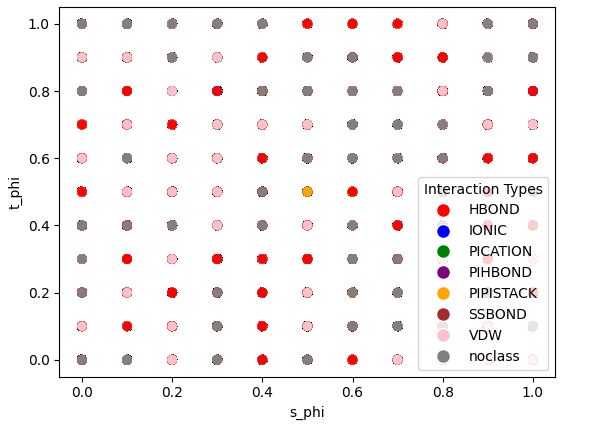
\includegraphics[scale=0.4]{img/scatterOriginalDS.png}
        \caption{Scatter plot of the dataset}
        \label{fig:scatterDataset}
    \end{figure}
\end{center}
\begin{center}
    \begin{figure}[h!]
        \centering
        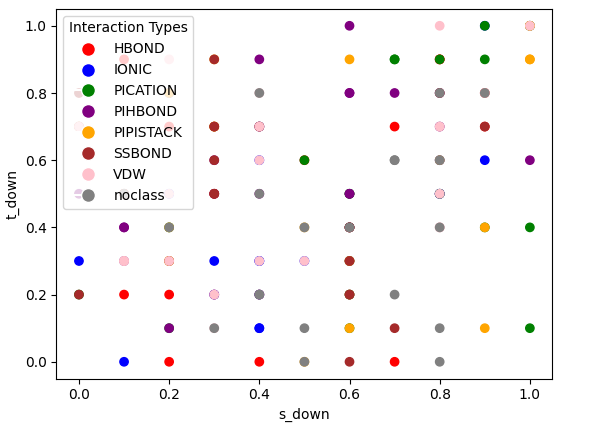
\includegraphics[scale=0.4]{img/ScatterSampled.png}
        \caption{Scatter plot of a sampled dataset}
        \label{fig:scatterSampled}
    \end{figure}
\end{center}

%inserire l'immagine con il plot dei dati

\subsection{XGBoost}
XGBoost\cite{DBLP:journals/corr/ChenG16} is an implementation of a gradient boosting\footnote{The boosting is an ensemble learning technique which 
imporove the performances of the model by combining weak model} algorithm and it constructs a series of decision
tree and improves the model each iteration. We tested this model both with the initial dataset and the dataset with the 
SMOTE applied.
\subsubsection{Parameter Selection}
The parameters that seemed most important to us in the modification were the following:
\begin{itemize}
    \item Max\_depth: this is the maximum depth of the tree, which is a crucial parameter to avoid overfitting. 
    It is setted to 10, which is a good compromise between the model's complexity and the risk of overfitting;
    \item Learning\_rate: setted to 0.1. This is the right value, an higher gives to us bad results and a lower 
    value makes the model too slow;
    \item num\_boost\_round: this is the number of iteration. It is setted to 2500. After 2500 iteration 
    is diffucult to see an improvement in the model;
    \item early\_stopping\_rounds: this is the number of iteration after which the model stops if it doesn't 
    improve. It is setted to 20.
\end{itemize}

\subsection{Neural Network Architecture}

The neural network model implemented in this project is a fully connected feedforward neural network, designed to classify protein residue interactions based on the features derived from the dataset. The architecture, named `SimpleNN`, consists of four layers, each with specific roles and activation functions chosen to optimize the model's performance on this multi-class classification task.

\subsubsection{Model Architecture}

The model consists of four fully connected layers: an input layer, two hidden layers, and an output layer. The hidden layers use ReLU activation functions to process and refine the features, while dropout layers are applied after each hidden layer to prevent overfitting. The final output layer uses a softmax activation function to produce probability distributions across the target classes, suitable for multi-class classification.

\subsubsection{Model Training}

For the training process, the Adam optimizer was employed alongside the Cross-Entropy loss function. 
The Adam optimizer was chosen due to its ability to efficiently handle large datasets and high-dimensional parameter spaces by adapting learning rates based on the estimates of first and second moments of the gradients. 
The Cross-Entropy loss function was selected because it effectively quantifies the difference between the predicted probabilities and the true class labels, making it well-suited for classification tasks.
Training was conducted using mini-batch gradient descent. 
For each mini-batch, predictions were computed, the loss was calculated, and the model weights were subsequently updated. This approach allows for more frequent updates and efficient handling of large datasets.

\subsection{Feature Importance and Feature Selection}
The model XGBoost is also capable of providing the importance of the features. It has three 
different methods to calculate the importance of the features: 
\begin{itemize}
    \item weight: total number of times a feature is used to split data across all trees;
    \item gain: average loss reduction gained when using a feature for splitting;
    \item cover: the number of times a feature is used to split data across trees weighted by training data points.
\end{itemize}
\begin{center}
    \begin{figure}[h!]
        \centering
        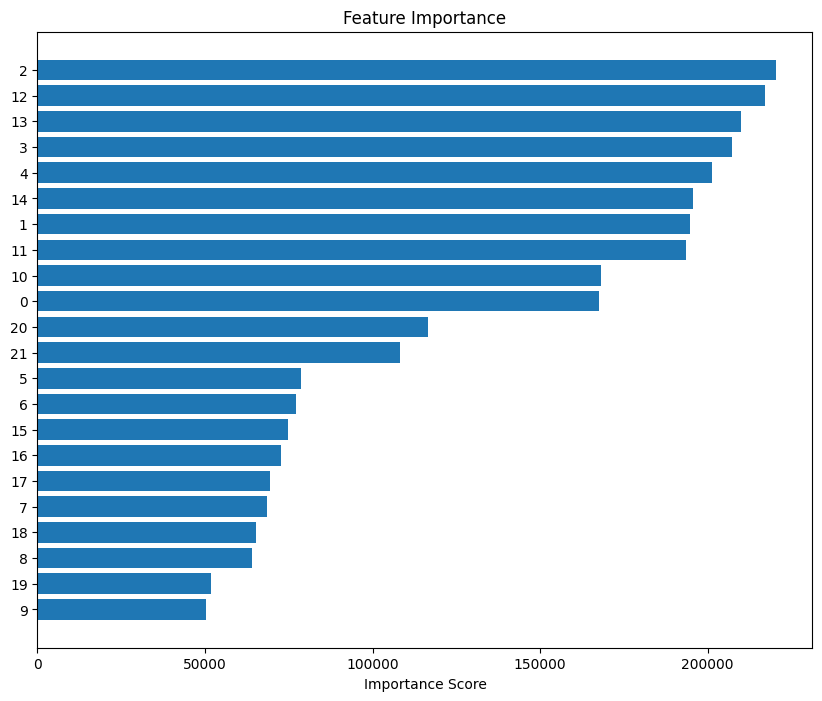
\includegraphics[scale=0.28]{img/fs.png}
        \caption{Feature importance given by XGBoost model (weight)}
        \label{fig:fs}
    \end{figure}
\end{center}
In the image \ref{fig:fs} we can see the score given to each feature and the importance of them 
for the classification of the interactions. The dataset has been modified by considering all the three method and a different number 
of feature for each type. The results were not better than the XGBoost model which used the dataset with SMOTE and which 
considered all the features.
\section{Model Evaluation Metrics}

The quality of the model was assessed using various evaluation metrics, including Matthews Correlation Coefficient (MCC), Balanced Accuracy, ROC-AUC, and Average Precision. These metrics were closely monitored throughout the training process to track the model's performance and progression.

\subsection{Rationale for Metric Selection}

The chosen metrics are particularly suited for handling imbalanced class distributions. Each metric provides distinct advantages in evaluating model performance:

\begin{itemize}
    \item \textbf{Matthews Correlation Coefficient (MCC):} MCC is a robust metric that considers true and false positives as well as true and false negatives, making it effective for evaluating the performance of models on imbalanced datasets. 
    Its ability to capture the balance between these quantities provides a comprehensive measure of classification quality;
    \item \textbf{Balanced Accuracy:} This metric calculates the average recall per class, addressing the issue of class imbalance by ensuring that each class contributes equally to the accuracy score. 
    Balanced Accuracy provides a more nuanced view of the model's performance across different classes, especially when some classes are underrepresented.;
    \item \textbf{ROC-AUC Score:} The ROC-AUC score evaluates the model's ability to distinguish between classes across all classification thresholds. 
    It is particularly useful for imbalanced datasets as it measures the overall capability of the model to rank positive instances higher than negative ones. A higher ROC-AUC score indicates better performance in differentiating between classes;
    \item \textbf{Average Precision:} The Average Precision score summarize the precision-recall curve as the weighted mean of precisions achieved at different threshold. 
    A high value of this metric indicates a better performance of the model in the classification 
    of the true positive instances.

\end{itemize}

Monitoring these metrics during training allows for a detailed assessment of the model's effectiveness and aids in the identification of potential areas for improvement, especially in the context of imbalanced datasets.

\section{Testing and results analysis}
The model has been trained on the 80\% of the dataset with the SMOTE applied and tested on the 20\% of the original dataset.
\begin{table}[h!]
    \centering
    \begin{tabular}{|p{1.6cm}|p{1.2cm}|p{1.2cm}|p{1.2cm}|p{1.2cm}|}
    \hline
    \textbf{Model} & \textbf{Bal Acc} & \textbf{MCC} & \textbf{AUC ROC} & \textbf{AVG Prec} \\
    \hline
    XGBoost (Initial DS) & 0.3669 & 0.2956 & 0.8741 & 0.5193 \\
    \hline
    \textbf{XGBoost (SMOTE)} & \textbf{0.5610} & \textbf{0.4752} & \textbf{0.9228} & \textbf{0.6704} \\
    \hline
    XGBoost (Feature Selection) & 0.5161 & 0.3554 & 0.8516 & 0.5080 \\
    \hline
    SimpleNN (SMOTE) & 0.4043 & 0.2321 & 0.7388 & 0.4432 \\ %inserire i valori
    \hline
    \end{tabular}
    \caption{Results of the models}
    \label{tab:results}
\end{table}

\subsubsection{Discussion}
The results reported show a substantial difference when dealing with SMOTE dataset and the initial one. Overall XGBoost 
performs well in both of them, but \textit{balanced accuracy}, \textit{MCC} and \textit{AVG precision} see an important 
improvement using SMOTE as we can see in the table \ref{tab:results}. 

The confusion matrix \ref{fig:cmXGBoostSMOTE} helps us understanding exactly where the model is doing wrong or right 
predictions. As we can see, the five less numerous classes are correctly classified by the model; thus the model is able 
to deal with the imbalance of the dataset. The problem arises when the model has to classify the three most prominent 
classes, because the '\textit{VDW}' bonds are really misleading for the right classification. 
That type of bonds are the worst classified of the entire dataset, leading to bad scores affecting the entire model. 
In fact, note that the True Positives for \textit{VDW} are around 40.000 examples while the \textit{VDW} classified as \textit{HBOND} are 50\% more numerous and the number of \textit{VDW} classified as \textit{noclass} is the 50\%.
\begin{center}
    \begin{figure}[h!]
        \centering
        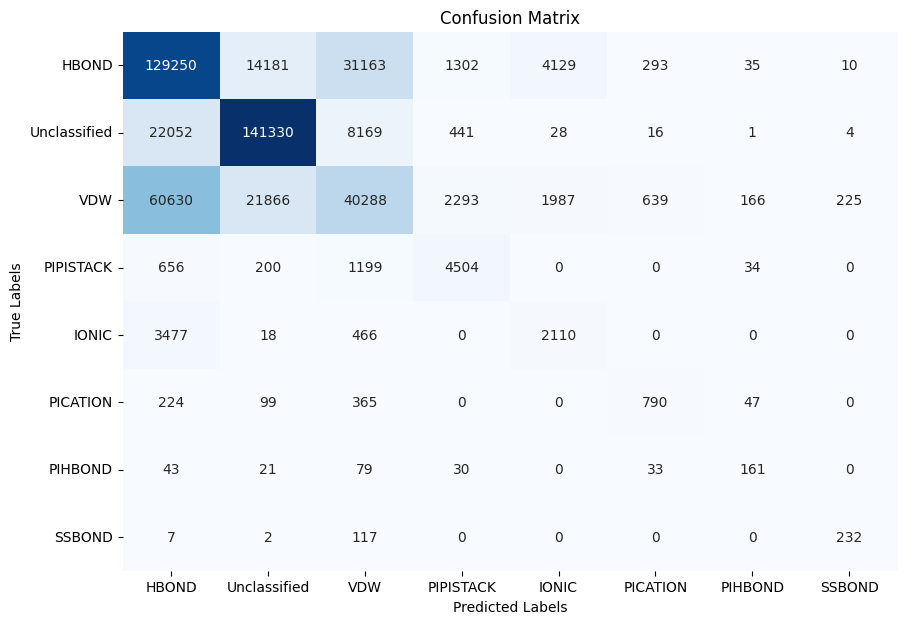
\includegraphics[scale=0.35]{img/cmXGBoostSMOTE.png}
        \caption{Confusion matrix of the XGBoost model with SMOTE}
        \label{fig:cmXGBoostSMOTE}
    \end{figure}
\end{center}

\section{Conclusions}
Finally we can say the best approach we've tried have been that one which uses the XGBoost 
with the SMOTE applied to the dataset as we can see in the table \ref{tab:results}. The model has a good performance in the classification of the 
interactions and the confusion matrix shows that the model is able to classify the interactions in a good way. 
The feature selection didn't give us better results than the model with all the features. 
The main problems have been the imbalance of the dataset and the overlap of the majority classes in the 
feature space. So, if we had more resources we could have thought of other more expensive approaches such as 
trying to project all the data in a higher dimension space in such a way as to better separate them.
{\small
\bibliographystyle{ieee_fullname}
\bibliography{egbib}
}

\end{document}
